 \thispagestyle{gocconone}
\pagestyle{gocco}
\everymath{\color{gocco}}
\graphicspath{{../gocco/pic/}}
\blfootnote{$^1${\color[named]{gocco}Trung tâm Quy hoạch và Điều tra tài nguyên -- môi trường biển khu vực phía Nam.}}
\begingroup
\AddToShipoutPicture*{\put(0,616){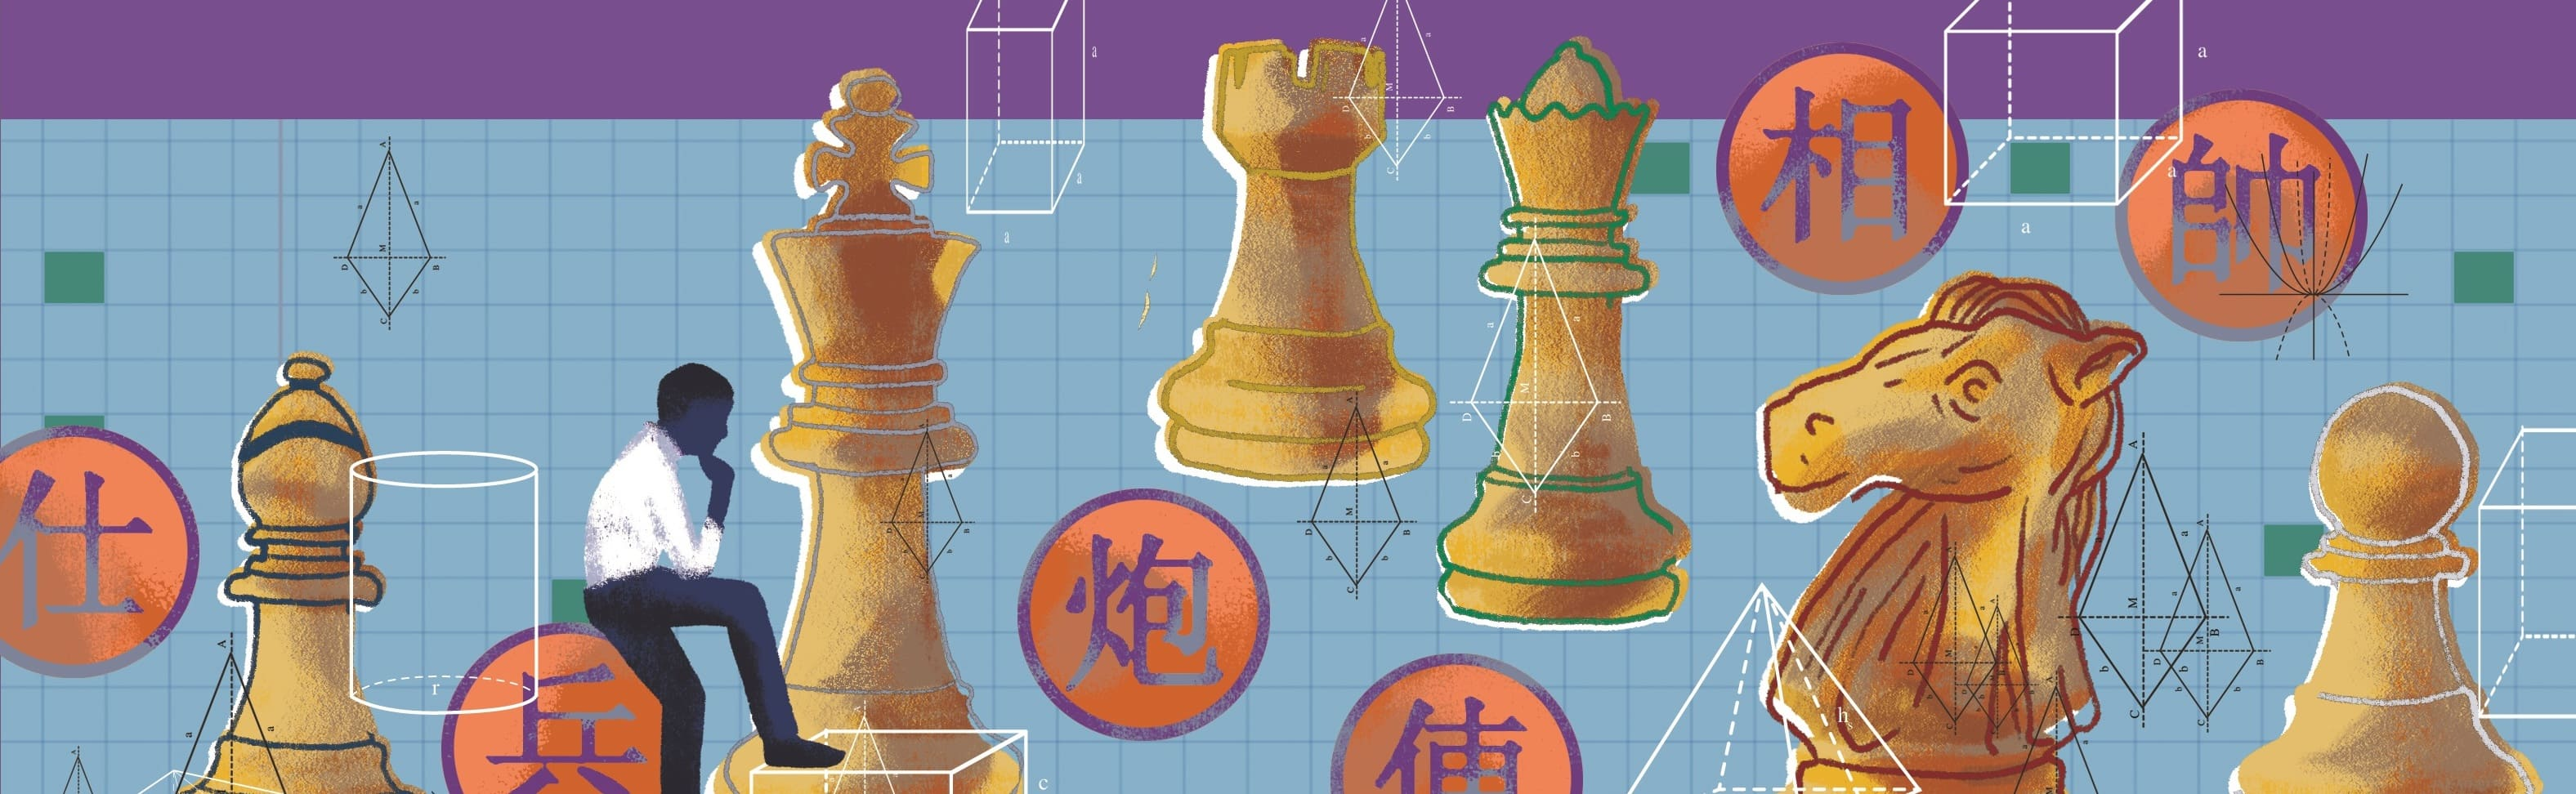
\includegraphics[width=19.3cm]{../bannergocco}}}
\AddToShipoutPicture*{\put(106,522){
\includegraphics[scale=1]{../tieude2.pdf}}} 
\centering
\endgroup

\vspace*{185pt}
\begin{multicols}{2}
	``\textit{Biết giấu mình dưới chín lớp đất cũng bằng biết khuấy động chín tầng trời}". Khi bắt đầu bước vào mỗi cuộc chiến cân não, nhiệm vụ quan trọng của đôi bên không chỉ là tìm cách bắt Tướng đối phương mà còn cần phải bảo vệ sự an toàn của Tướng của mình bằng những cách khéo léo và thông minh nhất. Để trở thành người chơi cờ giỏi, ngoài khả năng điều động quân lực, uy hiếp tấn công lên trận địa đối phương, các kỳ thủ cần sở hữu một kỹ năng không kém phần quan trọng, đó chính là Phòng thủ.
	\vskip 0.1cm
	Tuy vậy, tâm lý khi lâm trận của mỗi người thường muốn giành lấy chiến thắng càng nhanh càng tốt, nóng lòng hình thành thế tiến công ngay từ ban đầu khiến cho đối phương không kịp trở tay. Và nếu quá chăm chú vào mặt trận tấn tấn công mà lơ là mặt trận phòng thủ, hoặc phòng thủ một cách sơ sài, thiếu kế hoạch theo quan niệm ``\textit{Tấn công là cách phòng thủ tốt nhất}" thì chắc chắn sẽ để lộ ra những yếu điểm chết người, không thể giành thắng lợi mà còn tạo cơ hội cho đối phương phản kích dễ dàng.
	\vskip 0.1cm
	Trong bài viết kỳ này, tác giả sẽ gửi đến những hình cờ điển hình để bạn đọc Pi có thể hiểu hơn về tầm quan trọng của kỹ năng phòng thủ: 
	\vskip 0.1cm
	$1$.	Hình $1$, Đỏ còn chiến Xe rất mạnh và được đi tiên Đen chỉ còn Mã, Chốt và Tượng, Đỏ đi những nước mang tính uy hiếp như sau:  
	\begin{figure}[H]
		\vspace*{-5pt}
		\centering
		\captionsetup{labelformat= empty, justification=centering}
		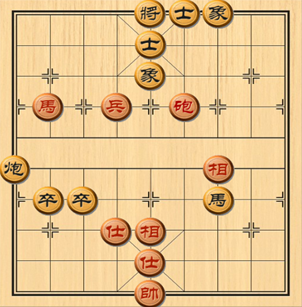
\includegraphics[width= 0.4\textwidth]{1}
		\caption{\small\textit{\color{gocco}Hình $1$.}}
		\vspace*{-10pt}
	\end{figure}
	$\pmb{1)}$	X$5-2$ M$3.5$\quad $\pmb{2)}$ X$2.6$ Tg$5.1$\quad $\pmb{3)}$ X$2/1$ Tg$5/1$\quad $\pmb{4)}$ X$2/1$ Tg$5.1$\quad $\pmb{5)}$ X$2/1$ M$5/7$\quad $\pmb{6)}$ X$2-3$ Tg$/1$\quad $\pmb{7)}$ X$3.1$ ($*$) Tg$.1$\quad $\pmb{8)}$ Tg$5.1$ M$3.5$ $(**)$  ($1/2$)
	\vskip 0.1cm
	\textit{$(*)$: Dựa vào sức mạnh tuyệt đối của Xe, Đỏ liên tục tung ra những đòn quấy rối cực kỳ khó chịu. Tương ứng với đó Đen cũng đưa ra những đáp trả rất chính xác.
	\vskip 0.1cm
	$(**)$: Nếu trong tình huống thông thường cũng với số lượng quân như vậy, Đỏ sẽ dễ dàng giành chiến thắng. Tuy nhiên với hình cờ cụ thể này, những quân của Đen đã có vị trí rất đẹp và vận dụng kỹ năng phòng thủ rất thuần thục, các quân liên kết một cách hợp lý, tạo ra bức tường không thể khoan phá. Ván đấu có kết quả hòa là hoàn toàn xác đáng.}
	\begin{figure}[H]
		\vspace*{-5pt}
		\centering
		\captionsetup{labelformat= empty, justification=centering}
		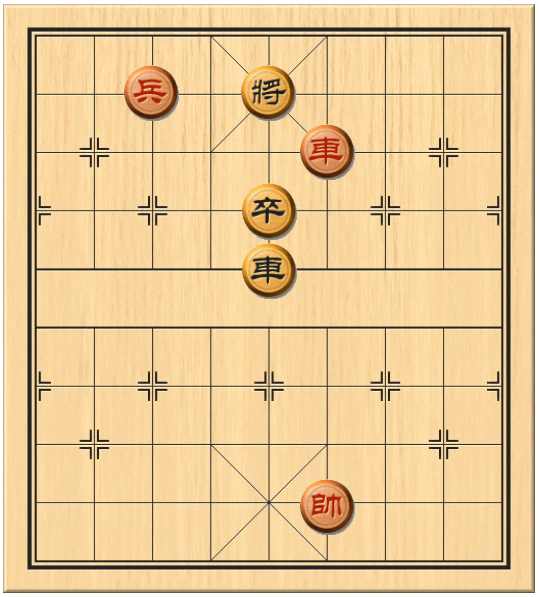
\includegraphics[width= 0.4\textwidth]{2}
		\caption{\small\textit{\color{gocco}Hình $2$.}}
		\vspace*{-10pt}
	\end{figure}
	$2.$ Hình $2$, đôi bên đang có quân lực như nhau, tuy nhiên Đỏ nắm lợi thế vì Xe Chốt đang áp sát, sẵn sàng lấy mạng Tướng đối phương bất cứ khi nào. Trong thế đi hậu liệu Đen có thể thủ hòa thành công ? Diễn biến tiếp theo của cuộc cờ như sau: 
	\vskip 0.1cm
	$\pmb{1)}$	X$4-6$ $(*)$ X$5-6$ \quad $\pmb{2)}$ Tg$4-5$ Tg$5-6$ $(**)$\quad $\pmb{3)}$ C$7-6$  X$6-8$ $(***)$\quad $\pmb{4)}$ X$6-5$ X$8-5$\quad $\pmb{5)}$ Tg$5-6$ X$5-4$\quad $\pmb{6)}$ Tg$6-5$ X$4/3$ $(****)$ ($1/2$)
	\vskip 0.1cm
	\textit{$(*)$: Với lợi thế đi tiên, Đỏ ngay lập tức bình Xe sang trục lộ $6$ hòng tạo điều kiện cho Chốt lộ $7$ xâm nhập cửu cung một cách dễ dàng hơn.
	\vskip 0.1cm
	$(**)$: Đen cũng không hề chịu thua kém, ngay lập tức bình Xe rồi bình Tướng qua trục còn lại chiếm con đường huyết mạch. 
	\vskip 0.1cm
	$(***)$: Mặc dù Đỏ có bình chốt áp sát, Đen vẫn bình tĩnh đưa Xe sang lộ $8$ -- một nước chờ đợi đầy kinh nghiệm. Nếu ở đây Đen vội vàng tấn Chốt nhằm tìm cơ hội đối công thì sẽ phải trả giá rất đắt, Đỏ đi X$4-5$, Đen thua ngay lập tức.
	\vskip 0.1cm
	$(****)$: Mặc dù Đỏ chỉ còn $1$ nước nữa là có thể bình Chốt tạo sát, nhưng Đen cũng có những nước đáp trả đầy mẫu mực. Đôi bên chỉ còn đơn Xe, ván đấu kết thúc với kết quả hòa.}
	\begin{figure}[H]
		\vspace*{-5pt}
		\centering
		\captionsetup{labelformat= empty, justification=centering}
		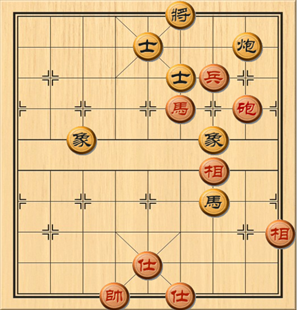
\includegraphics[width= 0.4\textwidth]{3}
		\caption{\small\textit{\color{gocco}Hình $3$.}}
		\vspace*{-10pt}
	\end{figure}
	$3.$ Hình $3$, Quân lực của Đỏ đang áp đảo nhưng Đen chỉ cần một nước nữa là có thể tạo ra sát cục. Trong tình thế cực kỳ nguy cấp, Đỏ đã liên tiếp tung ra những đòn phế quân để thủ hòa như sau:
	\vskip 0.1cm
	$\pmb{1)}$ Xt$.1$ S$5/4$\quad $\pmb{2)}$ X$6.2$ Tg$5.1$\quad $\pmb{3)}$ X$6-5$ Tg$5-6$\quad $\pmb{4)}$ M$5/3$ P$7/5$\quad $\pmb{5)}$ X$5/8$ $(*)$ P$7-4$\quad $\pmb{6)}$ P$3-6$ C$4-5$\quad $\pmb{7)}$ P$6-7$ C$5.1$ $(**)$\quad $\pmb{8)}$ P$7/5$ C$4-5$\quad $\pmb{9)}$ P$7-5$ $(***)$ ($1/2$)
	\vskip 0.1cm
	$(*)$: Trong thế không còn gì để mất, Đỏ đã liên tục bỏ quân, trước phế Xe, sau hiến Mã khiến cho Đen chưa thể kết thúc ván cờ. Tranh thủ thời gian quý báu đó, Đen lui về tiêu trừ Chốt $5$ của Đen và chiếm lấy vị trí đắc địa để phòng thủ.
	\vskip 0.1cm
	$(**)$: Dù đã mất quân Chốt quý giá, Đen vẫn đủ lực, sử dụng Pháo Chốt để tạo một đợt tấn công khác. Sau khi tấn Chốt chém Xe Đỏ, Đen tiếp tục dọa sát.
	\vskip 0.1cm
	$(***)$: Đen vẫn có những nước phòng thủ vô cùng hợp lý. Tuy vẫn còn một chút lợi thế nhưng chừng đó là chưa đủ để Đen giành chiến thắng.
	\vskip 0.1cm
	\textit{Chú thích}: C: Chốt, X: Xe, M: Mã, P: Pháo, Tg: Tướng, S: Sĩ, T: Tượng, t: trước.
	\vskip 0.1cm
	\textbf{\color{gocco}Câu đố kỳ này:}  Đôi bên sẽ vận dụng khả năng điều quân như thế nào để giữ vững trận địa trong những hình cờ đối công dưới đây (bên Đỏ được quyền đi trước)?
	\begin{figure}[H]
		\vspace*{-5pt}
		\centering
		\captionsetup{labelformat= empty, justification=centering}
		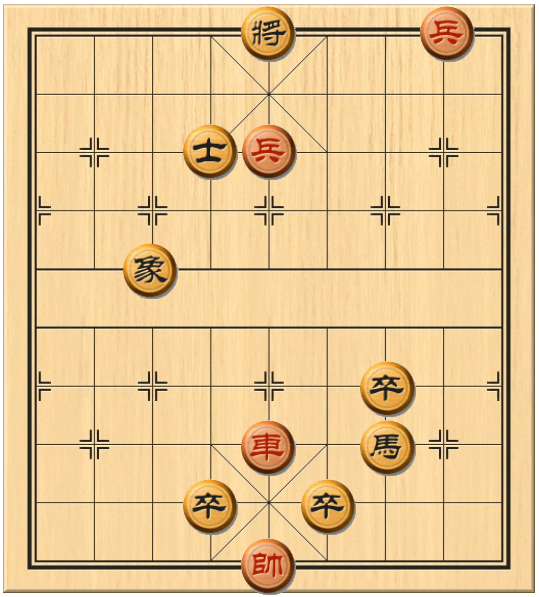
\includegraphics[width= 0.4\textwidth]{4}
		\caption{\small\textit{\color{gocco}Hình $4$.}}
		\vspace*{-10pt}
	\end{figure}
	\textit{Đáp án}: $\pmb{1)}$ C$5-6$ M$7/5$\quad $\pmb{2)}$ C$6.1$ T$3/5$\quad $\pmb{3)}$ C$2-3$ C$6-5$ \quad $\pmb{4)}$ Tg$5-4$ M$5.7$\quad $\pmb{5)}$ X$5-3$ C$5.1$\quad $\pmb{6)}$ Tg$4.1$ C$4-5$\quad $\pmb{7)}$ Tg$4-5$ C$7.1$ ($1/2$)
	\begin{figure}[H]
		\vspace*{-5pt}
		\centering
		\captionsetup{labelformat= empty, justification=centering}
		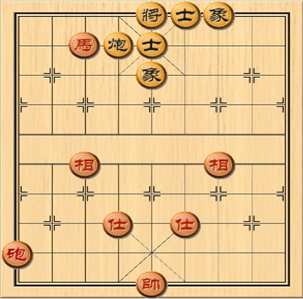
\includegraphics[width= 0.4\textwidth]{5}
		\caption{\small\textit{\color{gocco}Hình $5$.}}
		\vspace*{-10pt}
	\end{figure}
	\textit{Đáp án}: $\pmb{1)}$ X$4-5$ Tg$5.1$\quad $\pmb{2)}$ C$7-6$ X$4/1$\quad $\pmb{3)}$ C$4.1$ Tg$5/1$\quad $\pmb{4)}$ P$7.8$ S$4.5$\quad $\pmb{5)}$ C$4.1$ S$5/6$\quad $\pmb{6)}$ P$7-4$ Tg$5.1$\quad $\pmb{7)}$ X$8-5$ Tg$5/1$\quad $\pmb{8)}$ P$4-1$ Tg$5.1$\quad $\pmb{9)}$ P$1/1$ Tg$5/1$\quad $\pmb{10)}$ P$1-6$ Tg$5-4$ ($1/2$).
\end{multicols}




